\documentclass[12pt,a4paper]{scrartcl}

\newcommand{\Title}{{How to export a database from Filemaker}}

\title{\Title{}}
\date{8 Oct 2020}

\usepackage[utf8]{inputenc}
\usepackage[T1]{fontenc}

\usepackage[british]{babel}

\usepackage[sc]{mathpazo}
\usepackage[scaled=.9]{berasans}
\usepackage[scaled=.9]{beramono}

\usepackage{geometry}
\geometry{%
  includehead,includefoot,%
  top=2cm,bottom=2cm,%
  left=2cm,right=2cm,%
}

\usepackage{booktabs}
\usepackage{graphicx}

\usepackage{hyperref}
\hypersetup{%
  pdftitle=\Title,%
  pdfauthor=Johannes Englisch,%
  pdfborderstyle={/S/U/W 0},%
}


\begin{document}

\section{Introduction}%
\label{sec:intro}

Before data in a~Filemaker database can be converted into CLDF, we need to get
it out of the actual database.
Unfortunately there is no way to extract the data directly from the database
file, so it is necessary to export the data into an intermediate file format.

This document shows how to export all the views of the Filemaker database into
a~batch of separate Excel files.
These Excel files are then copied into the \emph{raw} folder of the
\emph{cldfbench} project and the conversion scripts will create the actual CLDF
from that.
% TODO github link to one of the cldfbenches, once they're public

% Mention the fact that this only works for a particular small set of databases
The Filemaker databases are organised in the following views:

\begin{itemize}
  \item \emph{Languages} (All languages in the database)
  \item \emph{Language parameters} (Questions one could ask about a~language)
  \item \emph{Language data} (Concrete answers to these questions for specific languages)
  \item \emph{Constructions} (All language-specific constructions in the database)
  \item \emph{Construction parameters} (Questions one could ask about a~construction)
  \item \emph{Construction data} (Concrete answers to these questions for specific constructions)
  \item \emph{Meanings} (Comparable meanings of constructions)
  \item \emph{Examples} (Example sentences)
  \item \emph{References} (Bibliographic information)
\end{itemize}

After the export, these views correspond the following files in the \emph{raw}
folder:

\begin{center}
  \framebox{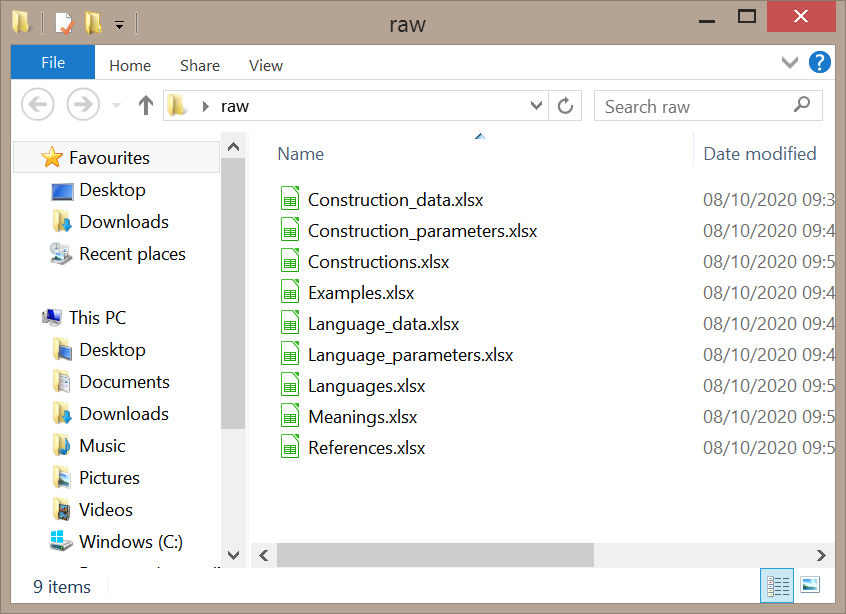
\includegraphics[scale=.6]{tutorial-images/raw-folder.png}}
\end{center}

Section~\ref{sec:howto} describes step by step, how a~view in Filemaker is
converted into an Excel spreadsheet.
Section~\ref{sec:columns} provides a~list of all columns that need to be
included in the spreadsheets for each view.


\section{How to export a view from Filemaker}
\label{sec:howto}

\begin{enumerate}
  \item
    Choose the view you want to export
    (e.\,g.\ \emph{Constructions (Editors' layout)}).\\[1ex]{}
    \framebox{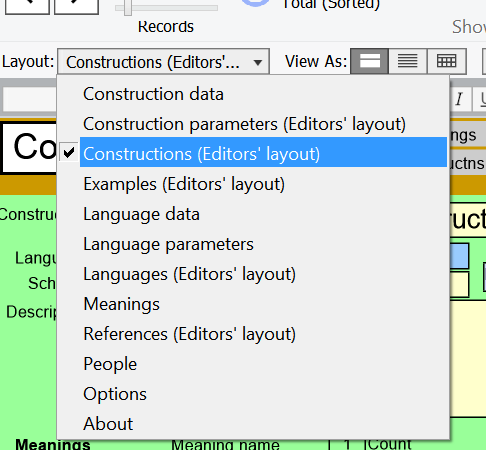
\includegraphics[scale=.6]{tutorial-images/01-choose-view.png}}

  \item
    The export yields a~different output, depending on how the data is currently
    displayed.
    So, for this export to work, set the view to a~single record using the
    \emph{View as} option.\\[1ex]{}
    \framebox{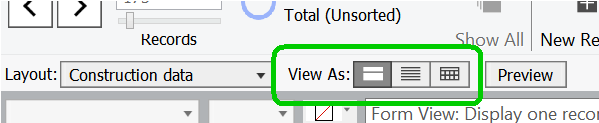
\includegraphics[scale=.6]{tutorial-images/02-view-as.png}}

    \newpage
  \item
    Also, the export does not include any data that is currently hidding, so
    to make sure \emph{all} data gets exported, click the \emph{Show All} button
    in the toolbar.\\[1ex]{}
    \framebox{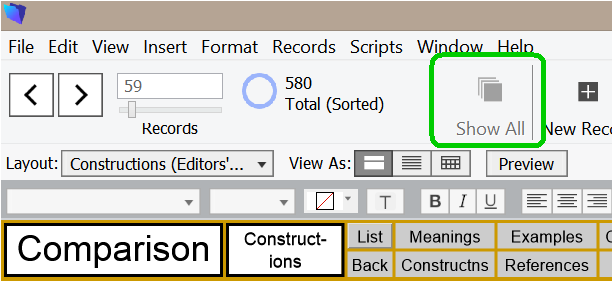
\includegraphics[scale=.6]{tutorial-images/03-show-all.png}}


  \item
    From the menubar choose \emph{File} $\to$ \emph{Export Records\dots}\\[1ex]{}
    \framebox{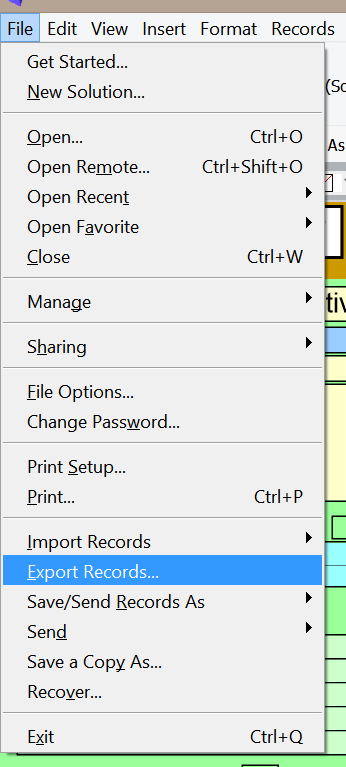
\includegraphics[scale=.6]{tutorial-images/04-export-menu.png}}

    \newpage
  \item
    In the upcoming file dialog, set the file type to \emph{Excel Workbooks
    (*.xlsx)} and choose the file name for the view as shown in
    Table~\ref{tab:filenames}.
    Note that the file names need to match the ones from the table
    \emph{exactly}.
    Even minor differences in punctuation or capitalisation may cause the
    conversion script to fail to recognise the files properly.\\[1ex]{}
    \framebox{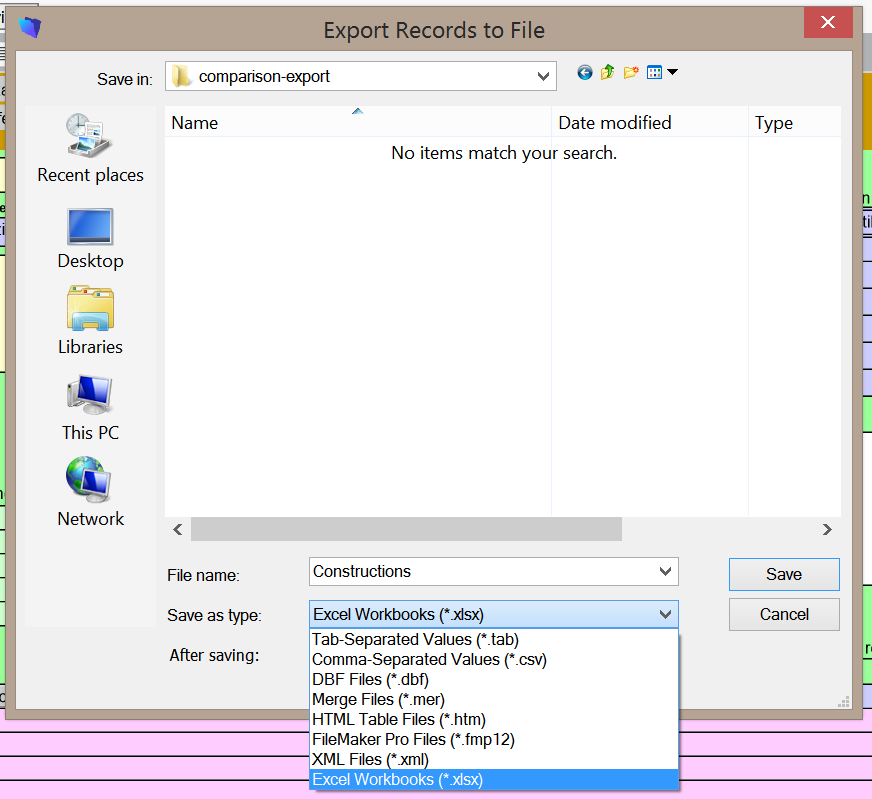
\includegraphics[scale=.6]{tutorial-images/05-export-dialog.png}}

    \begin{table}[ht]
      \centering%
      \begin{tabular}{lll}
        \toprule
        View                                      & File name \\\midrule
        Construction data                         & Construction\_data.xlsx \\
        Construction parameters (Editors' layout) & Construction\_parameters.xlsx \\
        Constructions (Editors' layout)           & Constructions.xlsx \\
        Examples (Editors' layout)                & Examples.xlsx \\
        Language data                             & Language\_data.xlsx \\
        Language parameters                       & Language\_parameters.xlsx \\
        Languages (Editors' layout)               & Languages.xlsx \\
        Meanings                                  & Meanings.xlsx \\
        References (Editors' layout)              & References.xlsx \\
        \bottomrule
      \end{tabular}
      \caption{Views in Filemaker and their corresponding Excel file names}%
      \label{tab:filenames}
    \end{table}

  \item
    In the following \emph{Excel Options} dialog, make sure the checkbox
    \emph{Use field names as column names in first row} is ticked.
    The other fields in the dialog can just be left blank.\\[1ex]{}
    \framebox{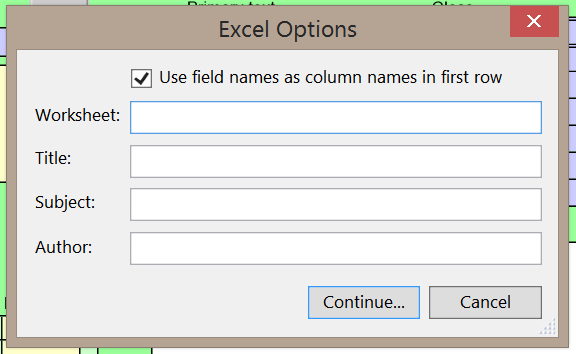
\includegraphics[scale=.6]{tutorial-images/06-excel-options.png}}

  \item
    Next Filemaker wants you to specify all table columns that should be
    exported.
    This dialog may contain settings from a~previous export.
    If you wish to remove those and start from scratch, hit the \emph{Clear All}
    button.\\[1ex]{}
    \framebox{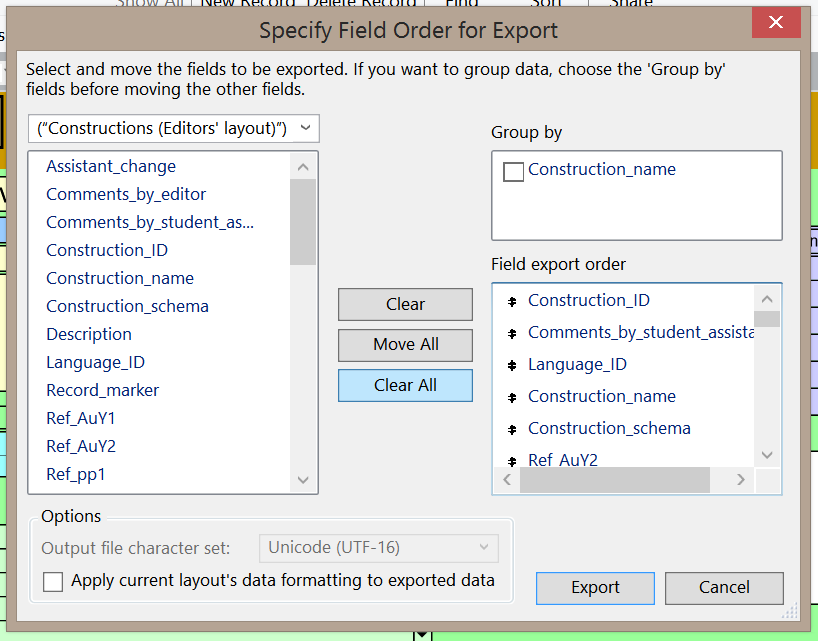
\includegraphics[scale=.6]{tutorial-images/07-clear-all.png}}

    \newpage
  \item
    To include table columns in the export, either double-click them in the left
    list or select them and hit the \emph{>> Move >>} button.
    For a~list of all columns that need to be included refer to
    Section~\ref{sec:columns} of this document.
    Note tha the exact order of columns is irrelevant to the conversion script.
    When you are done hit the \emph{Export} button to create the Excel
    export.\\[1ex]{}
    \framebox{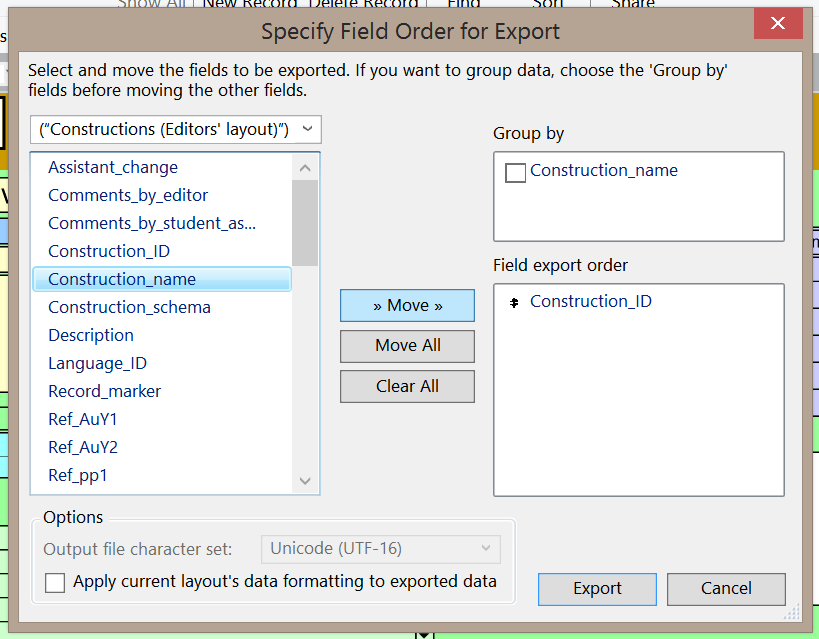
\includegraphics[scale=.6]{tutorial-images/08-move.png}}
\end{enumerate}


\newpage%
\section{Columns to be included in the export}%
\label{sec:columns}

\subsection{Construction data}

File name: Construction\_data.xlsx

\noindent\framebox{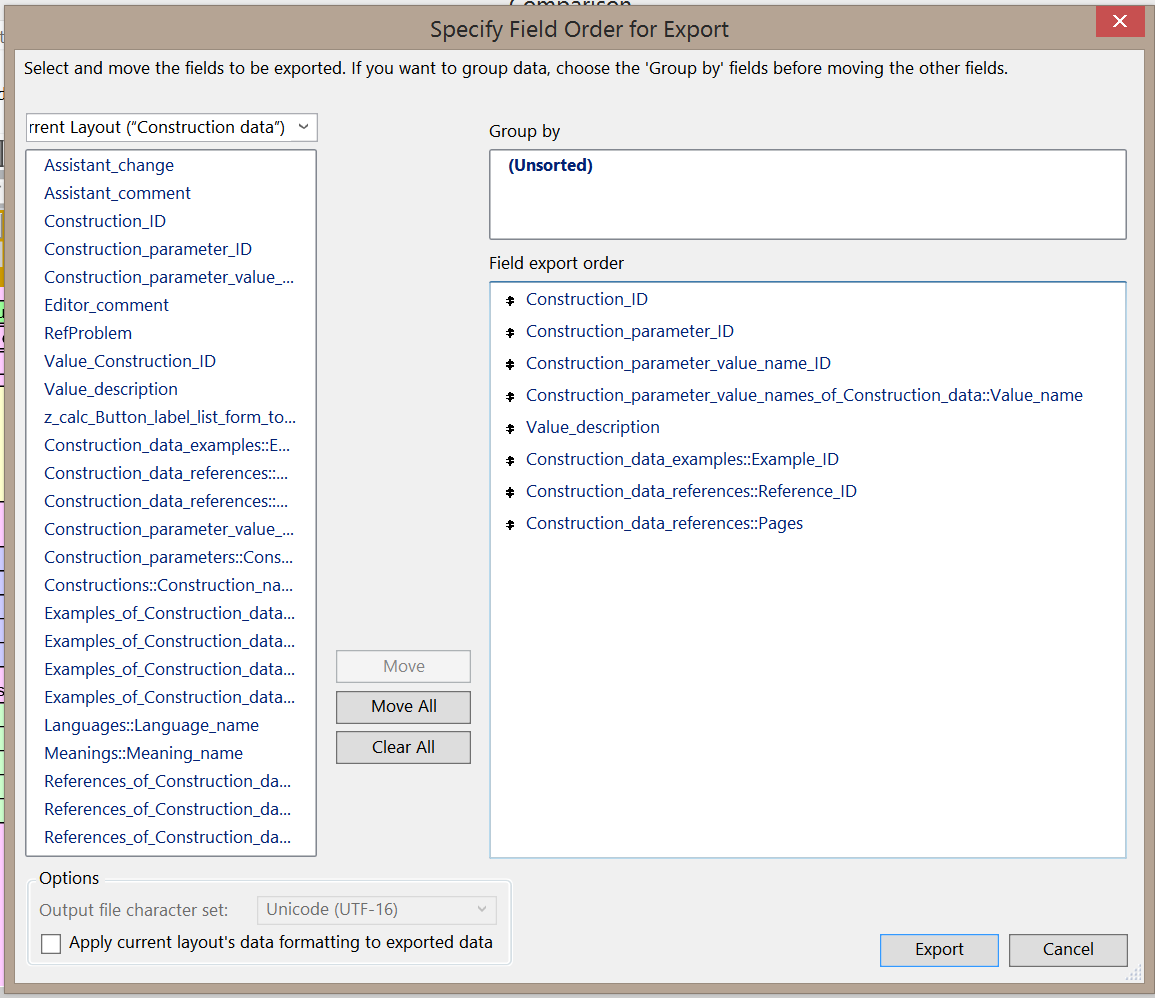
\includegraphics[scale=.5]{export-images/Construction_data.png}}

\newpage%
\subsection{Construction parameters}

File name: Construction\_parameters.xlsx

\noindent\framebox{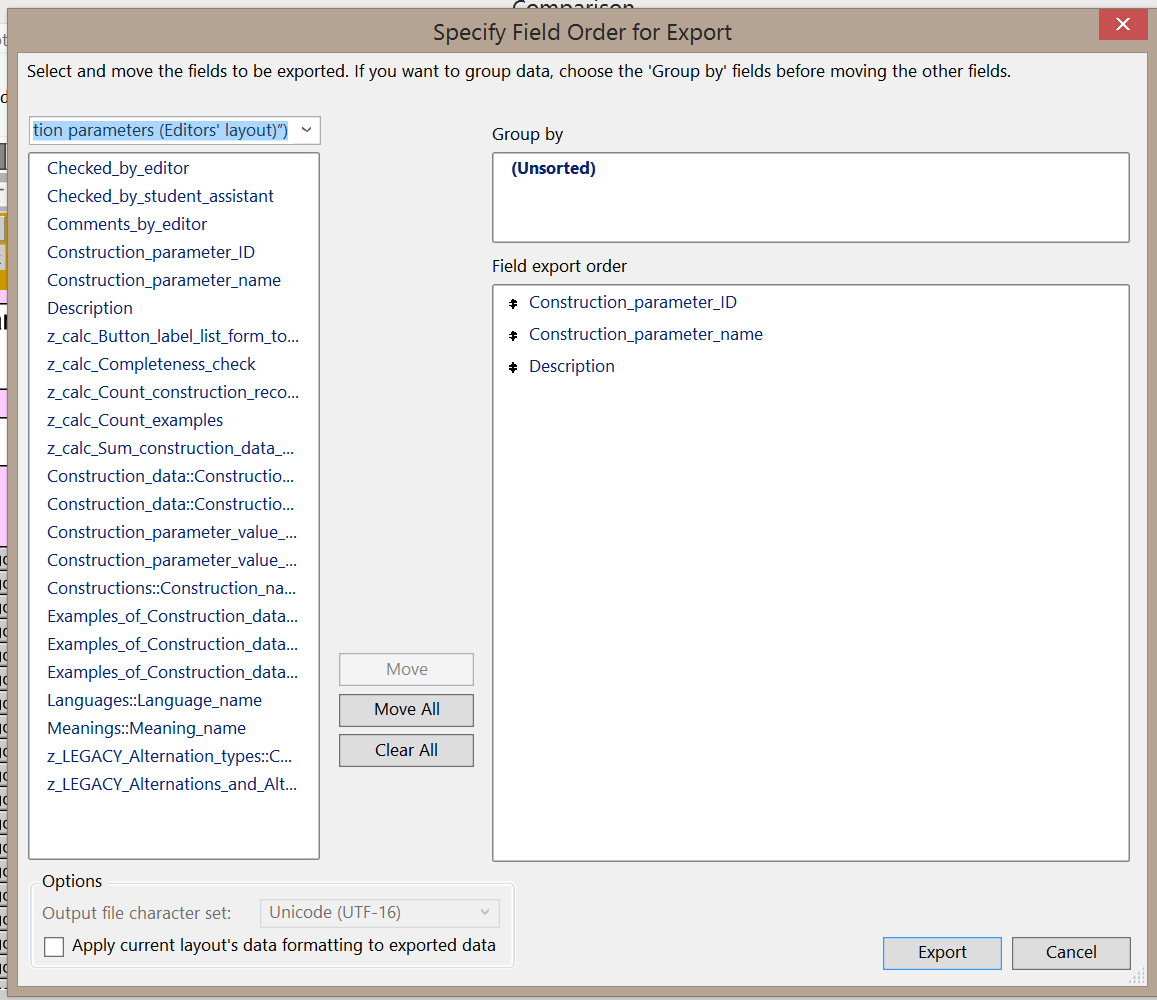
\includegraphics[scale=.5]{export-images/Construction_parameters.png}}

\newpage%
\subsection{Constructions}

File name: Constructions.xlsx

\noindent\framebox{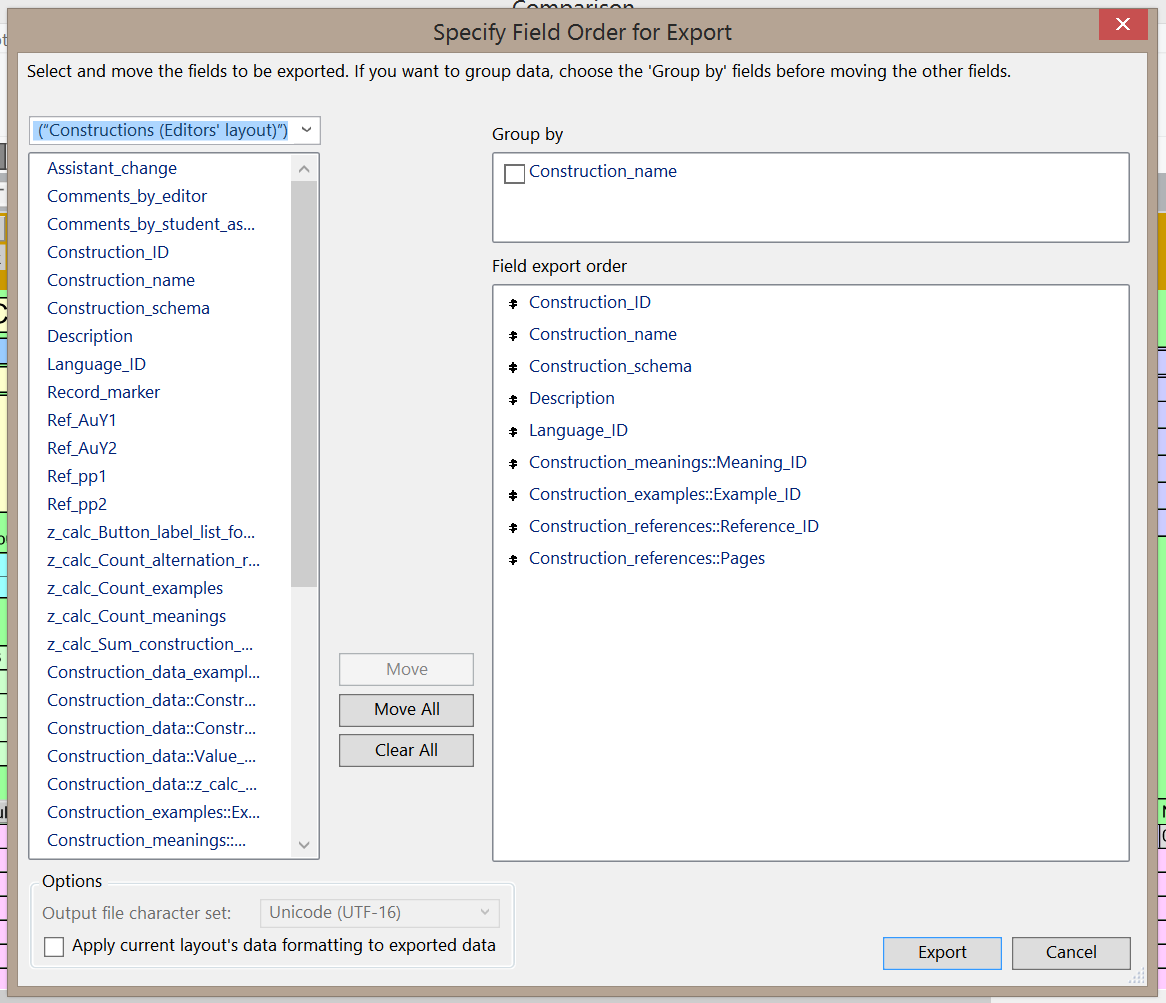
\includegraphics[scale=.5]{export-images/Constructions.png}}

\newpage%
\subsection{Examples}

File name: Examples.xlsx

\noindent\framebox{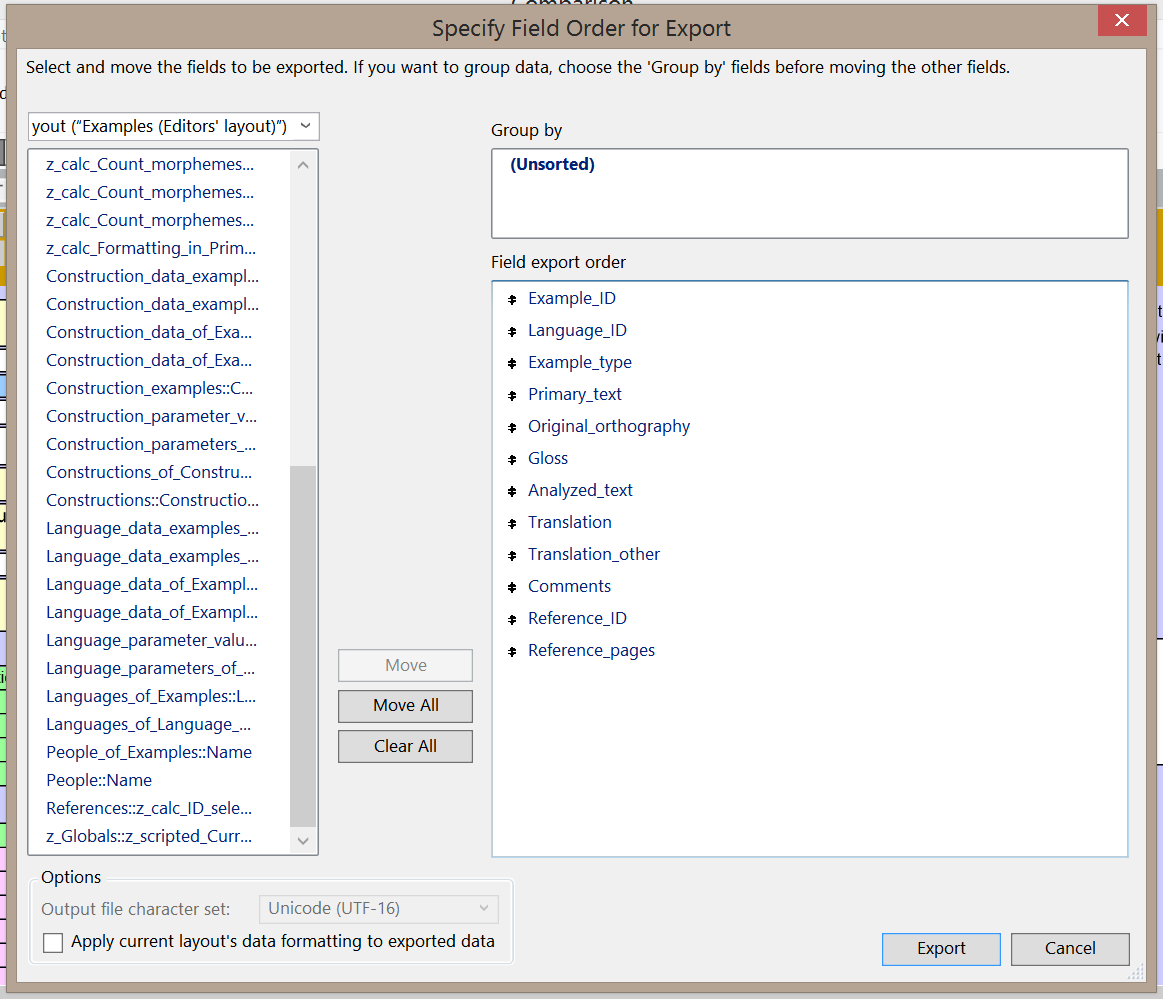
\includegraphics[scale=.5]{export-images/Examples.png}}

\newpage%
\subsection{Language data}

File name: Language\_data.xlsx

\noindent\framebox{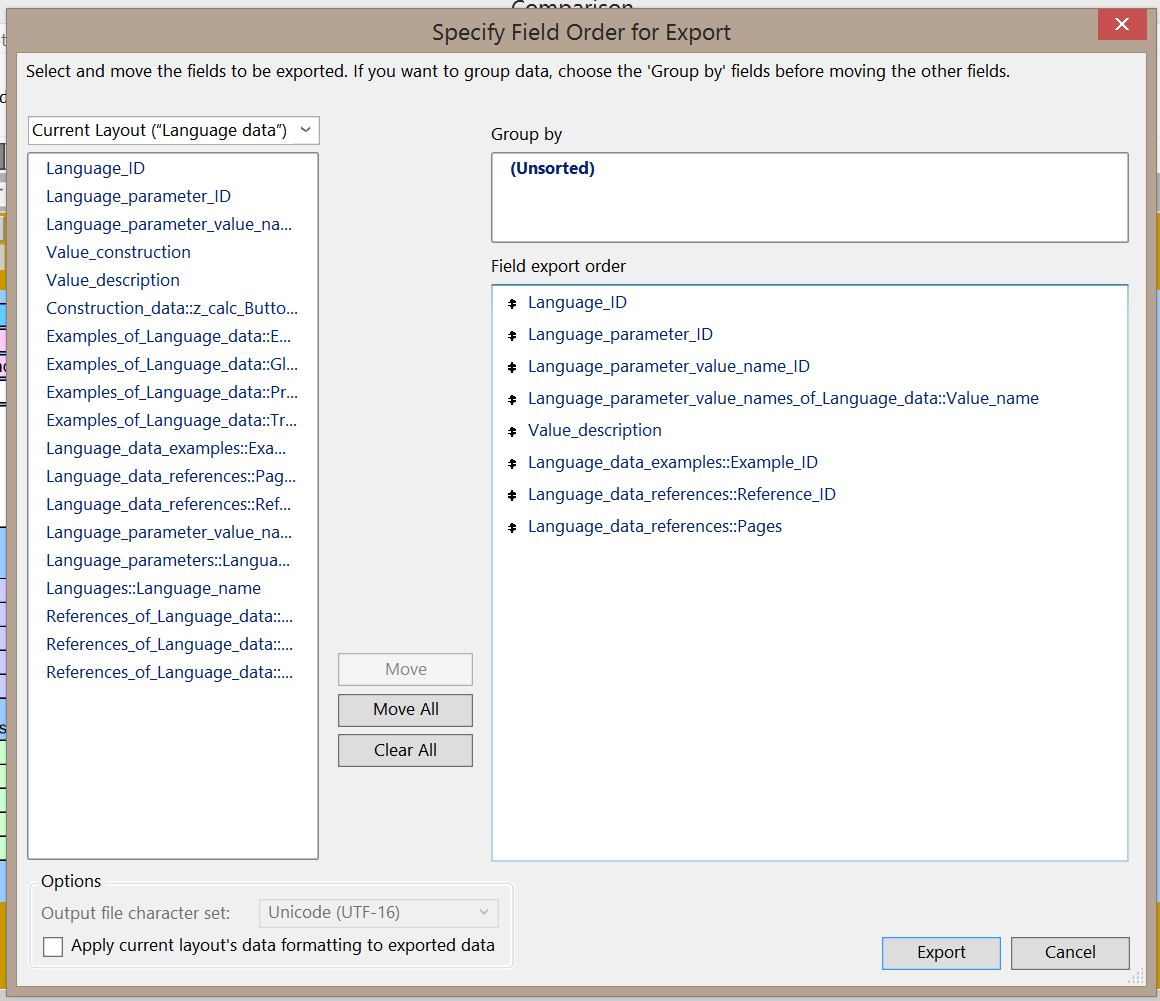
\includegraphics[scale=.5]{export-images/Language_data.png}}

\newpage%
\subsection{Language parameters}

File name: Language\_parameters.xlsx

\noindent\framebox{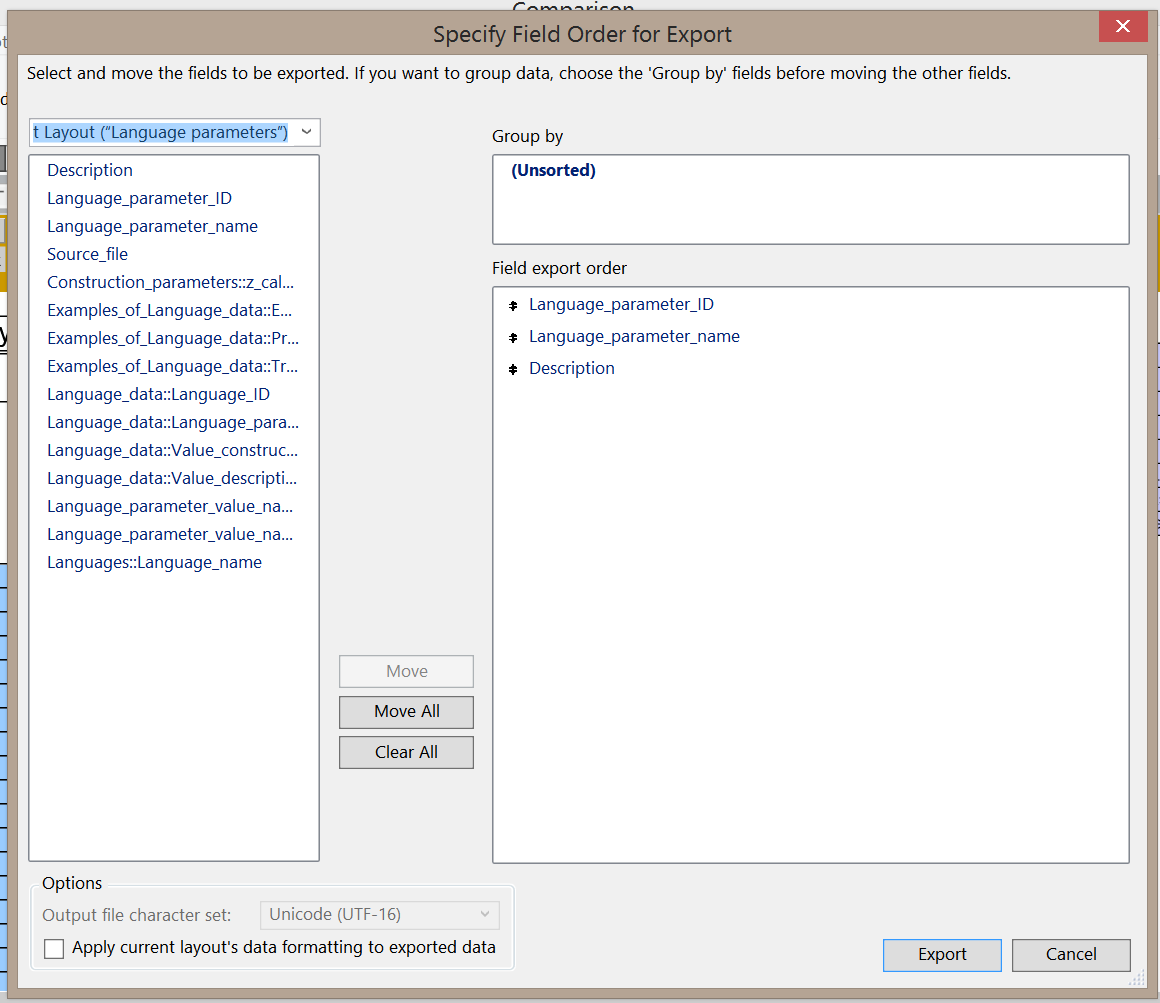
\includegraphics[scale=.5]{export-images/Language_parameters.png}}

\newpage%
\subsection{Languages}

Note that the language table is the most inconsistent across databases.
Some lack columns the \emph{Glottocode} or \emph{Language\_family}.
The conversion script will try and add missing information from the Glottolog.

File name: Languages.xlsx

\noindent\framebox{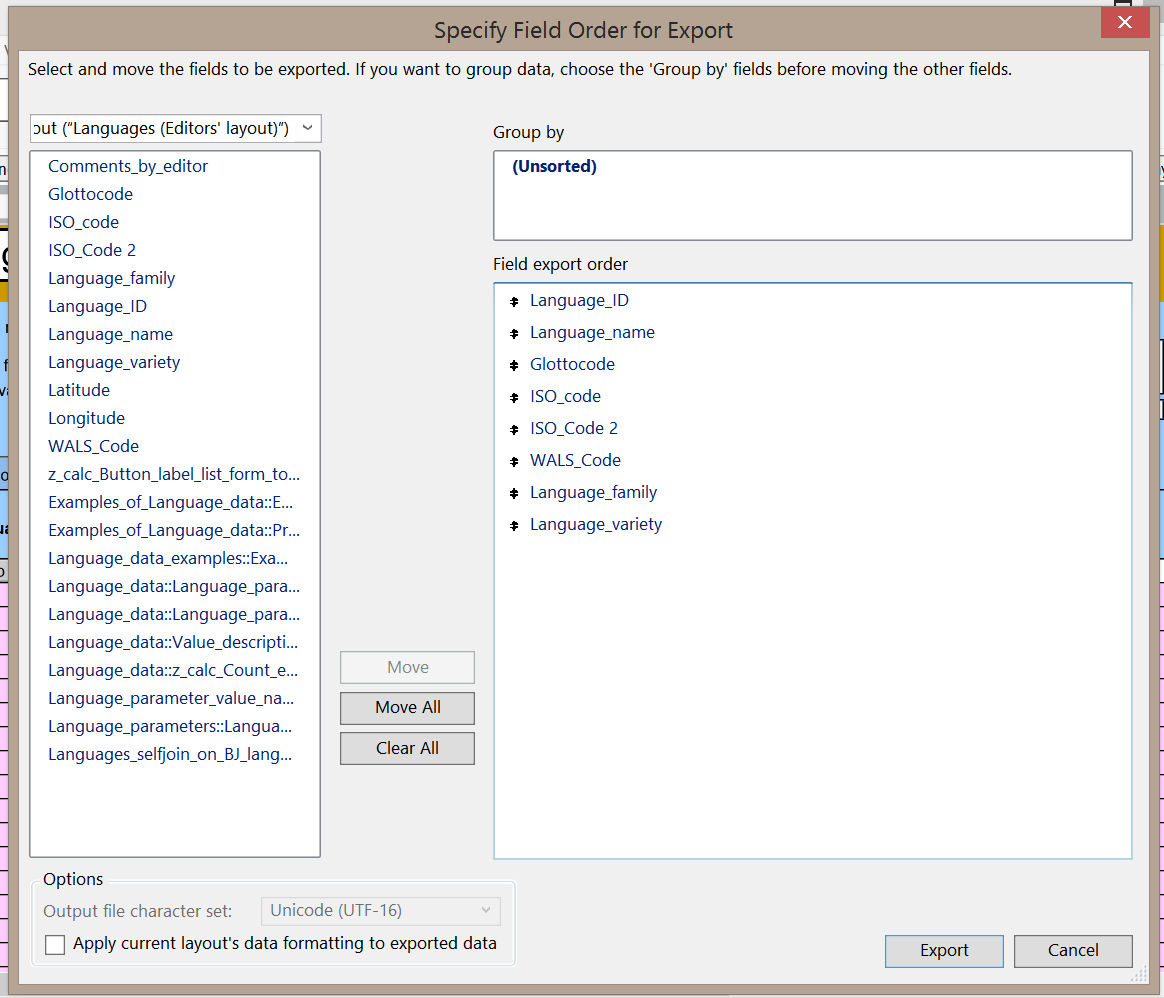
\includegraphics[scale=.5]{export-images/Languages-flagbase.png}}

\newpage%
\subsection{Meanings}

File name: Meanings.xlsx

\noindent\framebox{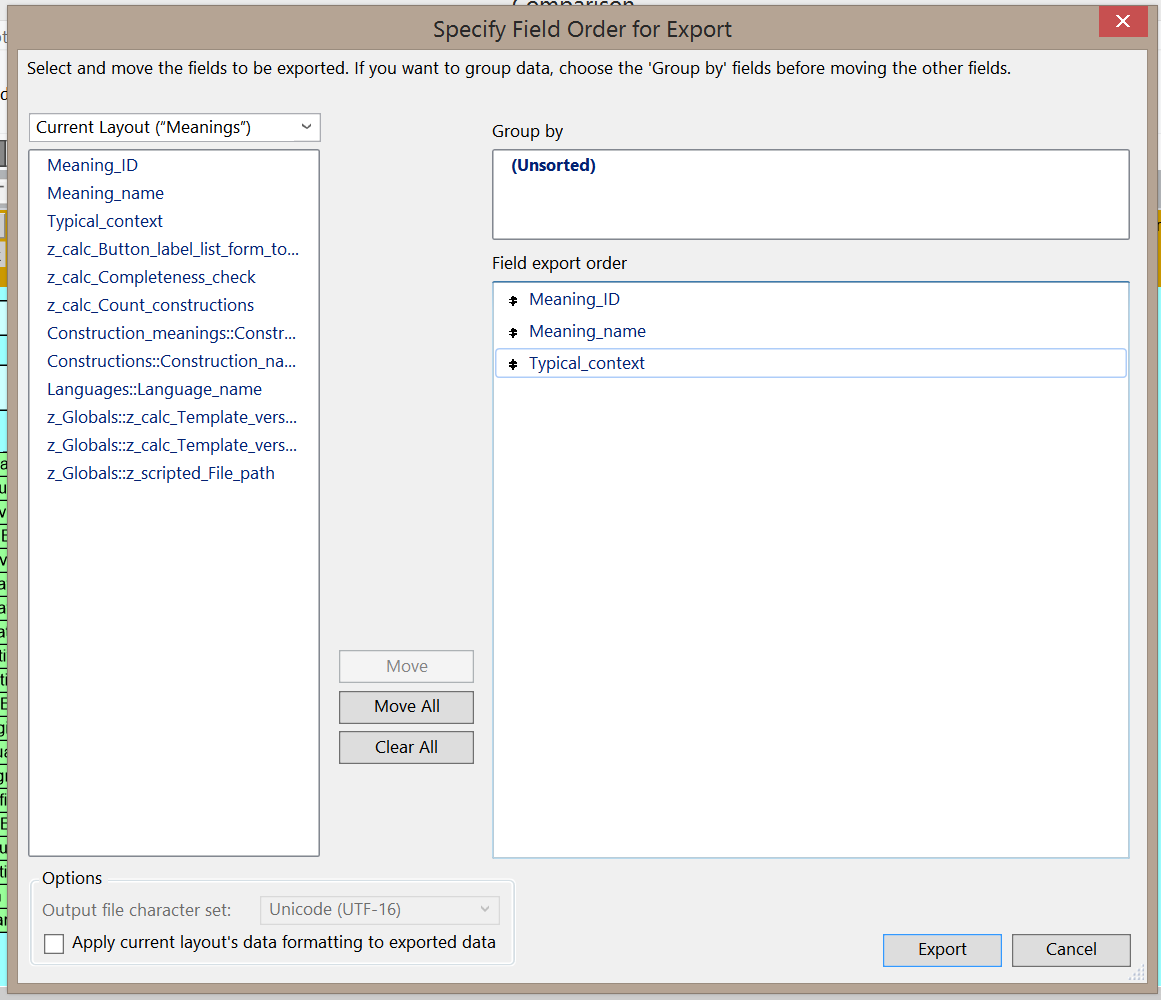
\includegraphics[scale=.5]{export-images/Meanings.png}}

\newpage%
\subsection{References}

File name: References.xlsx

\noindent\framebox{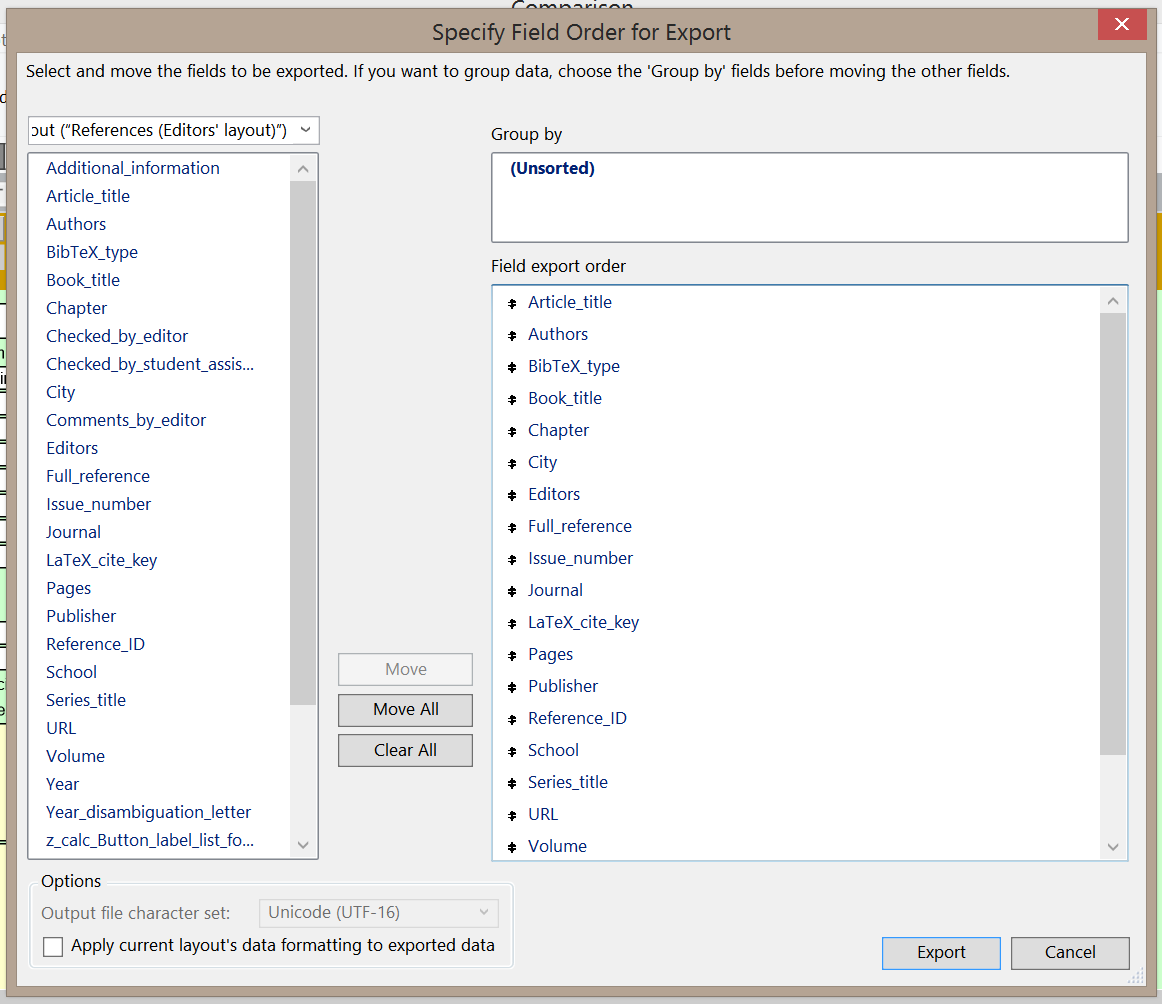
\includegraphics[scale=.5]{export-images/References-1.png}}

\noindent\framebox{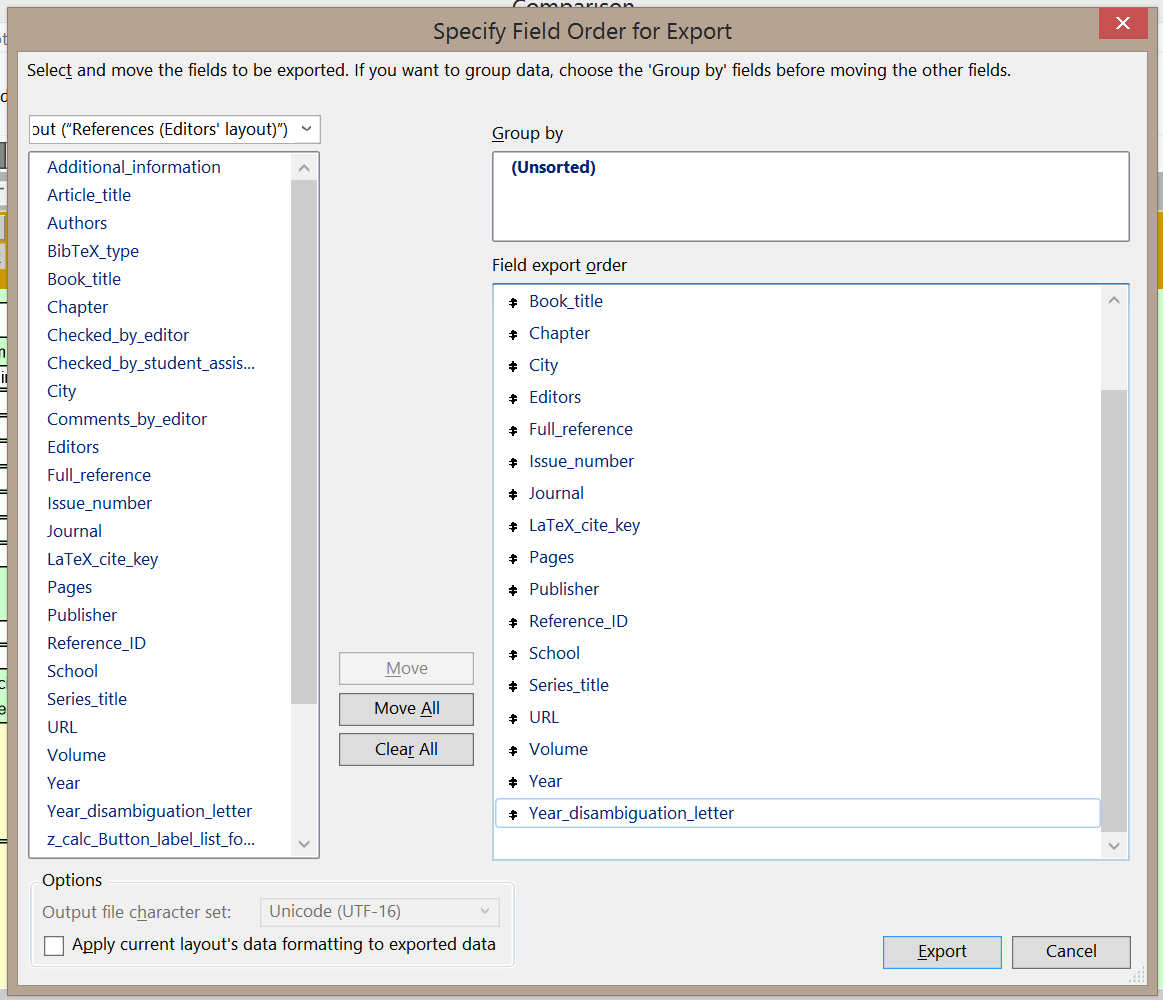
\includegraphics[scale=.5]{export-images/References-2.png}}

\end{document}
